\documentclass[11pt,a4paper]{article}
\usepackage[margin=2.42cm]{geometry}
\usepackage{amsmath,amssymb,amsthm,mathtools}
\usepackage{booktabs,array}
\usepackage{graphicx}
\usepackage{microtype}
\usepackage{xcolor}
\usepackage{hyperref}
\usepackage[nameinlink,noabbrev]{cleveref}
\usepackage[backend=biber,style=numeric-comp,sorting=none,maxbibnames=8]{biblatex}
\addbibresource{references.bib}

\hypersetup{
 colorlinks=true,
 linkcolor=blue!45!black,
 citecolor=blue!45!black,
 urlcolor=blue!55!black,
 pdftitle={Exact Classical Rate-Distortion for Phase-Lifted Generalized Coherent States: Cartan-Product Laplace Rigidity and Slater-Determinant Transitions},
 pdfauthor={Lluis Eriksson},
 pdfsubject={Information theory, representation theory, and coherent-state geometry},
 pdfkeywords={rate-distortion, generalized coherent states, Cartan product, Grassmannian, Slater determinant, phase transition}
}

\newtheorem{theorem}{Theorem}[section]
\newtheorem{proposition}[theorem]{Proposition}
\newtheorem{lemma}[theorem]{Lemma}
\newtheorem{corollary}[theorem]{Corollary}
\newtheorem{remark}[theorem]{Remark}
\newtheorem{definition}[theorem]{Definition}

\newcommand{\E}{\mathbb E}
\newcommand{\C}{\mathbb C}
\newcommand{\R}{\mathbb R}
\newcommand{\M}{\mathcal M}
\newcommand{\B}{\mathcal B}
\newcommand{\cP}{\mathcal P}
\newcommand{\cR}{\mathcal R}
\newcommand{\ip}[2]{\left\langle #1,#2\right\rangle}
\DeclareMathOperator{\conv}{conv}
\DeclareMathOperator{\cum}{cum}
\DeclareMathOperator{\Gr}{Gr}
\DeclareMathOperator{\Rea}{Re}

\title{\textbf{Exact Classical Rate--Distortion for Phase-Lifted\\
Generalized Coherent States}\\[2mm]
\large Cartan-product Laplace rigidity, universal radial envelopes,\\
and Slater-determinant transitions}
\author{Lluis Eriksson\\[-1mm]
\small Independent Researcher, Sweden\\
\small \href{mailto:lluiseriksson@gmail.com}{lluiseriksson@gmail.com}}
\date{August 14, 2026}

\begin{document}
\maketitle
\vspace{-1.3em}

\begin{abstract}
Let $V_\lambda$ be a finite-dimensional irreducible unitary representation
of a compact connected semisimple group, and let $X$ be uniform on the
phase-lifted orbit of a highest-weight vector.  We determine the classical
Shannon rate--distortion function of $X$ under squared ambient loss when the
description alphabet is arbitrary standard Borel and the decoder is not
restricted to the orbit.  The known integer-index generalized
Lieb--Wehrl theorem has a decisive information-theoretic consequence: a
Cartan-product identity makes coherent rays maximize the overlap Laplace
transform at every field and every fixed report norm.  The full vector
problem therefore reduces exactly to
\[
 C_\lambda(s)=e^{-s}\max_{0\le b\le1}
 e^{-sb^2}L_\lambda(2sb),\qquad
 L_\lambda(\kappa)=\sum_{m\ge0}
 \frac{(\kappa^2/4)^m}{(m!)^2\dim V_{m\lambda}},
\]
and $R_\lambda(D)=\sup_{s\ge0}\{-sD-\log C_\lambda(s)\}$.
Covariant tilted channels attain exposed points, while a revealed flag
mixing active radii attains every nonexposed point.  We derive a universal
representation-dimensional criterion for discontinuous directional-
information onset and a sharp root-system high-fidelity constant.  For
$V_\lambda=\Lambda^k\C^n$, the sources are phased fermionic Slater
determinants.  Their normalizer is an explicit ${}_{k-1}F_k$ function, their
squared Pl\"ucker overlap is a product of independent beta variables, and
every interior family $2\le k\le n-2$ with $n\ge6$ has a discontinuous first
activation.  A separate phase-invariant corollary gives the intrinsic
Pl\"ucker-distortion frontier on the projective coherent orbit.  These are
classical compression theorems for amplitude coordinates, not quantum
rate--distortion coding or a statement about click-only Born data.
\end{abstract}

\section{Introduction}

Generalized coherent states form the closed projective orbit of a
highest-weight ray.  They include spin coherent states, bosonic product
states, fermionic Slater determinants, and Pl\"ucker embeddings of complex
Grassmannians.  Their localization properties are governed by Wehrl and
R\'enyi--Wehrl moments.  Sugita proved that coherent states maximize every
integer Husimi moment for compact semisimple groups
\cite{Sugita2002}; the quadratic equality set is the highest-weight orbit
characterized by the Kostant--Lichtenstein quadrics
\cite{Lichtenstein1982,Baur2003}.  Those results are inputs here, not claims
of priority.

We ask a different question.  Draw a coherent state uniformly, attach an
independent phase, and encode the resulting vector using completely
classical memory.  How many nats are required to reconstruct it with a
prescribed squared Euclidean error if the decoder may report any vector,
not merely another coherent state?  The permission to leave the orbit is
substantive.  Conditional means live in the coherent-state orbitope and can
shrink radially; their competition produces linear faces and discontinuous
information onsets absent from a same-manifold codebook problem.

Rate--distortion on invariant groups and high-resolution bounds on
Grassmann manifolds are classical subjects
\cite{Harremoes2009,DaiLiuRider2008,RieglerKolianderBolcskei2023}.
For $V_\lambda=\C^n$ the phase-lifted source is exactly the real unit sphere
$S^{2n-1}$, and our $k=1$ formula reduces, with radius one and natural
logarithms, to the exact sphere solution of Dytso and Cardone
\cite{DytsoCardone2024}.  Quantum rate--distortion instead optimizes quantum
communication resources and quantum distortion observables
\cite{Barnum2000,KhanianWinter2022}; that is not the task considered here.

The paper's contribution begins after the known coherent-state moment
extremum.  We prove:
\begin{enumerate}
\item the all-field fixed-radius Laplace order obtained by positive
phase--Bessel resummation of Sugita's integer-moment extremum, together with
its exact equality classification;
\item an exact classical Shannon frontier over the full coherent-state
orbitope, including covariant equality and flagged attainment at
nonexposed distortions;
\item a universal criterion
$\dim V_{2\lambda}<\tfrac12(\dim V_\lambda)^2$ forcing a discontinuous first
activation;
\item a high-fidelity constant expressed directly by positive roots and the
highest weight;
\item an explicit all-$(n,k)$ Slater-determinant specialization with a
hypergeometric normalizer, beta-product overlap law, and a complete
classification of the sign responsible for first-order onset.
\end{enumerate}

The scalar formula is exact even when the radial maximizer is not unique.
We do not claim a unique positive branch or exclude later radial exchanges
for every representation.  That distinction keeps the result independent
of unproved phase-diagram assumptions.

\section{Coherent orbits and the unrestricted problem}

Let $G$ be a compact connected semisimple Lie group, let
$(\pi,V_\lambda)$ be a nontrivial finite-dimensional irreducible unitary
representation with dominant highest weight $\lambda$, and choose a unit
highest-weight vector $v_\lambda$.  We use the underlying real Hilbert
structure
\[
 (a,x)_\R=\Rea\ip{a}{x},\qquad \|a\|^2=\ip{a}{a}.
\]

\begin{definition}[Phase-lifted coherent orbit]
The source manifold and its orbitope are
\[
 \M_\lambda=\{e^{i\theta}\pi(g)v_\lambda:
 \theta\in\R/2\pi\mathbb Z,\ g\in G\},
 \qquad
 \B_\lambda=\conv(\M_\lambda).
\]
The probability $\mu_\lambda$ is the pushforward of normalized Haar
measure on $G$ and normalized Lebesgue measure on the phase circle.
\end{definition}

The independent phase makes $\E X=0$ for $X\sim\mu_\lambda$.  It also gives
$0\in\B_\lambda$, and convexity gives $\|a\|\le1$ for every
$a\in\B_\lambda$.

Let $Z$ take values in an arbitrary standard-Borel space and let
$a:Z\to V_\lambda$ be Borel.  We define
\[
 R_\lambda(D)=\inf I(X;Z),
 \qquad
 \E\|X-a(Z)\|^2\le D,
 \tag{2.1}
\]
where the infimum is over all joint laws with $X$-marginal
$\mu_\lambda$.  Mutual information and logarithms are in nats.

\begin{lemma}[Posterior-mean reduction]\label{lem:posterior}
The infimum in (2.1) is unchanged if the decoder is required to lie
in $\B_\lambda$.  More precisely, every decoder can be replaced by
\(\widehat X(Z)=\E[X\mid Z]\in\B_\lambda\) without increasing distortion
or mutual information.
\end{lemma}

\begin{proof}
Finite dimensionality makes the Bochner conditional expectation
well-defined.  Conditional least squares gives
\[
 \E[\|X-a(Z)\|^2\mid Z]
 =\E[\|X-\widehat X(Z)\|^2\mid Z]
  +\|a(Z)-\widehat X(Z)\|^2.
\]
The conditional mean belongs to the closed convex hull of the essential
range of $X$, which is $\B_\lambda$.  It is a measurable function of $Z$,
so data processing cannot increase mutual information.
\end{proof}

This unrestricted formulation is stronger than a codebook restricted to
$\M_\lambda$.  The report can be a proper mixture of coherent states, but
\cref{thm:laplace} will show that only one radial coherent direction is
needed in the dual optimum.

\section{Cartan products and all-field Laplace rigidity}

Let $V_{m\lambda}$ denote the irreducible Cartan component generated by
$v_\lambda^{\otimes m}$ inside $V_\lambda^{\otimes m}$, let
$P_{m\lambda}$ be its orthogonal projector, and write
\[
 d_m=d_m(\lambda)=\dim V_{m\lambda},\qquad d_0=1.
\]

\begin{lemma}[Cartan moment identity]\label{lem:cartan}
For every $a\in V_\lambda$ and integer $m\ge1$,
\[
 \int_G|\ip{a}{\pi(g)v_\lambda}|^{2m}\,dg
 =\frac{\|P_{m\lambda}a^{\otimes m}\|^2}{d_m}
 \le\frac{\|a\|^{2m}}{d_m}.
 \tag{3.1}
\]
For $a\ne0$, equality at $m=2$ holds exactly when $[a]$ lies on the
projective highest-weight orbit.
\end{lemma}

\begin{proof}
The vectors $(\pi(g)v_\lambda)^{\otimes m}$ span $V_{m\lambda}$.  The
operator
\[
 T_m=\int_G |(\pi(g)v_\lambda)^{\otimes m}\rangle
 \langle(\pi(g)v_\lambda)^{\otimes m}|\,dg
\]
vanishes on the orthogonal complement and commutes with the irreducible
$G$-action on $V_{m\lambda}$.  Schur's lemma makes it a scalar multiple of
$P_{m\lambda}$; its trace is one, so $T_m=P_{m\lambda}/d_m$.  Contracting
with $a^{\otimes m}$ gives the identity and the projection bound.  For
$m=2$, equality says $a^{\otimes2}\in V_{2\lambda}$.  The
highest-weight quadratic criterion identifies precisely the coherent rays
\cite{Lichtenstein1982}.  This is also the projection proof underlying the
integer-index generalized Lieb--Wehrl theorem \cite{Sugita2002}.
\end{proof}

Define the entire even function
\[
 L_\lambda(\kappa)=\sum_{m=0}^\infty
 \frac{(\kappa^2/4)^m}{(m!)^2d_m}.
 \tag{3.2}
\]
Convergence follows already from $d_m\ge1$ and comparison with
$I_0(|\kappa|)$.

\begin{theorem}[All-field coherent-ray rigidity]\label{thm:laplace}
For every $a\in V_\lambda$ and real $\kappa$,
\[
 \int_{\M_\lambda}
 e^{\kappa\Rea\ip{a}{x}}\,d\mu_\lambda(x)
 \le L_\lambda(\kappa\|a\|).
 \tag{3.3}
\]
Equality holds for every scalar multiple of a coherent vector.  If
$\kappa\|a\|\ne0$, equality forces $a$ to lie on a coherent ray.
\end{theorem}

\begin{proof}
For $z\in\C$, phase averaging gives
\[
 \frac1{2\pi}\int_0^{2\pi}
  (\Rea(e^{i\theta}z))^{2m}\,d\theta
 =\frac{\binom{2m}{m}}{4^m}|z|^{2m},
\]
and all odd moments vanish.  Expand the exponential, apply
\cref{lem:cartan}, and use
$\binom{2m}{m}/(2m)!=1/(m!)^2$.  Every term is nonnegative.  Coherent
$a$ saturates each projection inequality.  Conversely, equality of the
sum at a nonzero argument forces equality of its $m=2$ term, and the final
claim follows from \cref{lem:cartan}.
\end{proof}

The theorem is an all-field consequence of known integer moment rigidity.
It is useful because exponential loss duals require the entire transform,
not a fixed R\'enyi index.

\section{Exact Shannon rate--distortion}

For $s\ge0$ and $a\in\B_\lambda$ of norm $b$,
\[
 \int e^{-s\|x-a\|^2}\,d\mu_\lambda(x)
 =e^{-s(1+b^2)}
   \int e^{2s\Rea\ip{a}{x}}\,d\mu_\lambda(x).
 \tag{4.1}
\]
Because $bv_\lambda\in\B_\lambda$ for $0\le b\le1$,
\cref{thm:laplace} makes the supremum exact.

\begin{theorem}[Universal coherent-orbit RDF]\label{thm:rdf}
Put
\[
 C_\lambda(s)=e^{-s}\max_{0\le b\le1}
 \left\{e^{-sb^2}L_\lambda(2sb)\right\}.
 \tag{4.2}
\]
Then
\[
 \boxed{
 R_\lambda(D)=\sup_{s\ge0}\{-sD-\log C_\lambda(s)\}.}
 \tag{4.3}
\]
This identity holds for arbitrary standard-Borel classical descriptions
and all $D\ge0$.  In particular, $R_\lambda(D)=0$ for $D\ge1$.

At every exposed point, an active radius $b$ is attained by a covariant
tilted channel supported on $b\M_\lambda$.  At a nonexposed point, a
revealed independent flag mixing at most two active radii attains the
frontier.
\end{theorem}

\begin{proof}
We give the standard-Borel converse and equality construction explicitly.
By \cref{lem:posterior}, assume from the outset that every report
$a_z$ lies in $\B_\lambda$.
Regular conditional laws $\nu_z=P_{X\mid Z=z}$ exist.  For every report
$a_z$ and $s\ge0$, the entropy variational inequality gives, with extended
values,
\[
 D(\nu_z\|\mu_\lambda)
 +s\E_{\nu_z}\|X-a_z\|^2
 \ge-\log\int e^{-s\|x-a_z\|^2}\,d\mu_\lambda(x)
 \ge-\log C_\lambda(s).
 \tag{4.4}
\]
Averaging and using
$I(X;Z)=\E_ZD(P_{X\mid Z}\|\mu_\lambda)$ yields
$I(X;Z)\ge-sD-\log C_\lambda(s)$.  Optimization in $s$ proves the lower
bound.  This is the constant Shannon dual written without a hidden finite-
alphabet or absolute-continuity assumption
\cite{Berger1971,Csiszar1974}.

Fix a maximizing radius $b$ and let $Y$ be Haar on $\M_\lambda$.  Define
the reverse kernel
\[
 \frac{dP_{X\mid Y=y}}{d\mu_\lambda}(x)
 =\frac{e^{-s\|x-by\|^2}}{C_\lambda(s)}.
 \tag{4.5}
\]
The denominator is correct because $b$ is active.  Averaging the numerator
over $y$ gives a $G\times U(1)$-invariant function of $x$ and is therefore
constant on the transitive source orbit.  Its integral is
$C_\lambda(s)$, so the $X$-marginal of the joint law is exactly
$\mu_\lambda$.  Reporting $A=bY$, direct evaluation gives
\[
 I(X;Y)=-sD_b-\log C_\lambda(s),
 \qquad D_b=\E\|X-bY\|^2.
 \tag{4.6}
\]
For an interior active radius, differentiation of
$K_\lambda(2sb)-sb^2$ gives
\[
 b=K_\lambda'(2sb).
 \tag{4.7}
\]
The gradient of the log partition at a fixed-norm coherent maximizer is
radial, and its radial component is $K_\lambda'(2sb)$; hence
$\E[X\mid Y=y]=by$.  Thus the displayed report is also the posterior mean.
At $b=0$ the same statement follows from phase symmetry; $b=1$ is excluded
at finite field below.
Thus every distortion in $-\partial\log C_\lambda(s)$ is attained.  If
several radii are active, choose an independent revealed flag $J$ and use
the corresponding kernel conditionally on $J$.  Each component has the
same $X$-marginal, hence $I(X;J)=0$ and both distortion and conditional
mutual information mix linearly.  One-dimensional convexity requires at
most two radii.

At $s=0$, $b=0$ gives $D=1$ and zero rate.  As $s\to\infty$, active radii
approach one and the distortion approaches zero; this follows also from the
high-field estimate in \cref{prop:highfield}.  Convex closure supplies the
endpoints and completes Fenchel equality.
\end{proof}

An equivalent primal form is useful for geometry.  Define the Cram\'er
transform and its squared-radius parametrization by
\[
 j_\lambda(b)=\sup_{\kappa\ge0}
 \{\kappa b-K_\lambda(\kappa)\},\qquad
 g_\lambda(u)=j_\lambda(\sqrt u),\quad 0\le u<1.
 \tag{4.8}
\]

\begin{corollary}[Convex-envelope form]\label{cor:convex-envelope}
For $0\le D\le1$,
\[
 R_\lambda(D)=(\operatorname{co}g_\lambda)(1-D),
 \tag{4.9}
\]
where $\operatorname{co}$ denotes the lower convex envelope.  Every chord
is attained by time sharing between two covariant coherent tilts.
\end{corollary}

\begin{proof}
For a posterior law $\nu$ with mean $a$ and $b=\|a\|$, entropy variation
with the field $\kappa a/b$ and \cref{thm:laplace} gives
$D(\nu\|\mu_\lambda)\ge j_\lambda(b)$.  Conditional means satisfy
$\E\|X-\E[X\mid Z]\|^2=1-\E b(Z)^2$.  The function
$\operatorname{co}g_\lambda$ is nonnegative, convex, vanishes at zero, and
is therefore nondecreasing.  Jensen's inequality consequently gives
\[
 \E g_\lambda(b(Z)^2)
 \ge \E(\operatorname{co}g_\lambda)(b(Z)^2)
 \ge (\operatorname{co}g_\lambda)(1-D),
\]
which is the converse.  Conversely, a coherent exponential
tilt of parameter $\kappa$ has mean
$K_\lambda'(\kappa)y$, divergence
$j_\lambda(K_\lambda'(\kappa))$, and the invariant source marginal after
Haar mixing of $y$.  Strict convexity makes $K_\lambda'$ increasing;
phase symmetry gives $K_\lambda'(0)=0$.  The high-field estimate in
\cref{lem:saddle} gives $K_\lambda(\kappa)/\kappa\to1$, and convexity then
forces $K_\lambda'(\kappa)\to1$ without differentiating its remainder.  Hence it maps
$\kappa\in[0,\infty)$ onto $b\in[0,1)$, so all points of $g_\lambda$ are
attained.  A revealed binary flag mixing two such joint laws preserves the
same source marginal, is independent of $X$, and attains every lower-hull
chord.
\end{proof}

\begin{remark}[Finite-field boundary]
The endpoint $b=1$ is not active at finite $s>0$.  Writing
$K=\log L$ and differentiating the radial objective gives
$2s[K'(2sb)-b]$.  Under every finite coherent tilt the overlap is strictly
less than one almost surely, so $K'(2s)<1$; moving left from $b=1$ strictly
increases the objective.
\end{remark}

\section{A representation-dimensional phase criterion}

The radial problem is
\[
 \phi_s(b)=K_\lambda(2sb)-sb^2,
 \qquad K_\lambda=\log L_\lambda.
 \tag{5.1}
\]
The zero report always has value zero.  Its quadratic stability changes at
$s_0=\dim V_\lambda$.

\begin{proposition}[Fourth-cumulant criterion]\label{prop:cumulant}
Let $N=d_1=\dim V_\lambda$.  For
$Y=\Rea\ip{v_\lambda}{X}$,
\[
 \E Y^2=\frac1{2N},\qquad
 \cum_4(Y)=\frac38\left(\frac1{d_2}-\frac2{N^2}\right).
 \tag{5.2}
\]
If $d_2<N^2/2$, the first global activation of a nonzero report occurs at
some $s_c<N$ with a radius bounded away from zero.  Hence $R_\lambda$ has a
linear coexistence face adjacent to $D=1$ and a discontinuous onset of
directional information.
\end{proposition}

\begin{proof}
The moments follow from \cref{lem:cartan} and phase averaging.  Since
\[
 K_\lambda(t)=\frac{t^2}{4N}
 +\frac{\cum_4(Y)}{24}t^4+O(t^6),
\]
the coefficient of $b^2$ in (5.1) is
$s(s/N-1)$.  Thus $b=0$ is a strict local maximum for $0<s<N$.  At $s=N$
the quadratic term vanishes; if $\cum_4(Y)>0$, every sufficiently small
nonzero $b$ has $\phi_N(b)>0$.  For small $s>0$, zero is the unique global
maximizer: $|\Rea\ip{a}{X}|\le\|a\|$ and Hoeffding's lemma give
$K_\lambda(2sb)\le2s^2b^2$, so $\phi_s(b)<0$ for $0<s<1/2$ and $b>0$.
Compactness and continuity therefore give an attained first contact
$0<s_c<N$.

Were positive maximizers at contact to converge to zero, the locally
uniform expansion at $s_c<N$ would make $\phi_s(b)<0$ for all sufficiently
small nonzero $b$, a contradiction.  The contact radius is therefore
positive.  Mixing the zero and positive covariant channels in
\cref{thm:rdf} produces the linear face.
\end{proof}

This criterion proves existence, not uniqueness, of coexistence.  A global
one-fold theorem requires additional information about the full dimension
sequence $d_m$ and is deliberately not assumed.

\section{Root-system high-fidelity asymptotics}

Let $\rho$ be the Weyl vector and let
\[
 \Phi_\lambda^+=\{\alpha>0:
 \ip{\lambda}{\alpha^\vee}>0\},\quad
 p=|\Phi_\lambda^+|,\quad
 A_\lambda=\prod_{\alpha\in\Phi_\lambda^+}
 \frac{\ip{\rho}{\alpha^\vee}}{\ip{\lambda}{\alpha^\vee}}.
 \tag{6.1}
\]
The projective coherent orbit has real dimension $2p$; its phase lift has
dimension $q=2p+1$.

\begin{lemma}[Bessel-weighted polynomial saddle]\label{lem:saddle}
Suppose $d_m$ is given by Weyl's formula for $V_{m\lambda}$.  Then, with
$a=p+1/2$,
\[
 L_\lambda(\kappa)=
 \frac{2^pA_\lambda}{\sqrt{2\pi}}
 e^\kappa\kappa^{-a}(1+o(1)),
 \tag{6.2}
\]
\end{lemma}

\begin{proof}
Weyl's dimension formula is
\[
 d_m=\prod_{\alpha>0}
 \frac{m\ip{\lambda}{\alpha^\vee}+\ip{\rho}{\alpha^\vee}}
      {\ip{\rho}{\alpha^\vee}}
 =\frac{m^p}{A_\lambda}(1+O(m^{-1})).
 \tag{6.3}
\]
Put $z=\kappa/2$ and let $M_z$ have probability masses
\[
 \Pr\{M_z=m\}=\frac{z^{2m}}{(m!)^2I_0(2z)}.
 \tag{6.4}
\]
If $N_1,N_2$ are independent $\operatorname{Poisson}(z)$ variables, then
$M_z\overset d=N_1\mid\{N_1=N_2\}$.  For fixed
$0<\epsilon<1$, Poisson Chernoff bounds and Stirling's lower bound at
$m_0=\lfloor z\rfloor$ give
\[
 \Pr(|N_1-z|>\epsilon z)\le2e^{-c_\epsilon z},
 \qquad
 \Pr(N_1=N_2)\ge\Pr(N_1=m_0)^2\ge c z^{-1}.
 \tag{6.5}
\]
Consequently
\[
 \Pr(|M_z-z|>\epsilon z)\le C z e^{-c_\epsilon z}.
 \tag{6.6}
\]
The Weyl asymptotic in (6.3) is uniform on every tail interval.
On $|M_z-z|\le\epsilon z$, it squeezes $z^p/d_{M_z}$ between quantities
converging to $A_\lambda$ as first $z\to\infty$ and then
$\epsilon\downarrow0$.  On the complement, $d_m^{-1}\le1$ and
(6.6) is exponentially smaller than $z^{-p}$; the $m=0$ mass is
also exponentially small.  Hence
\[
 \E d_{M_z}^{-1}\sim A_\lambda z^{-p}.
 \tag{6.7}
\]
Finally
$L_\lambda(2z)=I_0(2z)\E d_{M_z}^{-1}$ and
$I_0(2z)\sim e^{2z}/\sqrt{4\pi z}$, which proves (6.2) with the
displayed constant.  This drifting-saddle argument is uniform and does not
interchange an unbounded limit with a merely pointwise Weyl estimate.
\end{proof}

\begin{proposition}[Sharp high-fidelity constant]\label{prop:highfield}
As $D\downarrow0$,
\[
 \boxed{
 R_\lambda(D)=
 \frac q2\log\frac qD-\frac q2
 -\log\left(\frac{2^pA_\lambda}{\sqrt{2\pi}}\right)+o(1).}
 \tag{6.8}
\]
\end{proposition}

\begin{proof}
By \cref{lem:saddle},
$K(\kappa)=\kappa-(q/2)\log\kappa+
\log(2^pA_\lambda/\sqrt{2\pi})+o(1)$.
Put $a=q/2$, $C=2^pA_\lambda/\sqrt{2\pi}$, and
$t=\delta\kappa$.  Uniformly for $t$ in compact subsets of
$(0,\infty)$,
\[
 \kappa(1-\delta)-K(\kappa)
 =a\log(1/\delta)+a\log t-t-\log C+o(1).
\]
The deterministic function $a\log t-t$ has its unique maximum at $t=a$.
The same asymptotic excludes $t\to\infty$ and excludes $t\to0$ whenever
$\kappa\to\infty$, while bounded $\kappa$ gives only $O(1)$ and cannot
compete with the diverging value $a\log(1/\delta)$.  Hence
$\delta\kappa_\delta\to a$ and direct Legendre optimization gives
\[
 j_\lambda(1-\delta)=
 \frac q2\log\frac{q/2}{\delta}-\frac q2
 -\log\left(\frac{2^pA_\lambda}{\sqrt{2\pi}}\right)+o(1).
\]
Since $D=1-b^2=2\delta+o(\delta)$, this is (6.8) on the
deterministic-radius curve.  Lower convexification does not improve its
leading term.  Indeed, for a mixed squared radius $U$ put
$\Delta=1-U$ and assume $\E\Delta=D$.  On
$A_D=\{\Delta\le\sqrt D\}$, Markov gives
$P(A_D)=1-o(1)$ and the preceding asymptotic is uniform.  Conditional
Jensen for $-\log\Delta$ yields
\[
 P(A_D)\E[-\log\Delta\mid A_D]
 \ge P(A_D)\log\frac{P(A_D)}{\E[\Delta;A_D]}
 \ge P(A_D)\log\frac{P(A_D)}D
 =\log(1/D)+o(1).
\]
The complement contributes nonnegatively.  This gives the matching lower
bound, while the deterministic choice gives the upper bound.  No
differentiation of the $o(1)$ saddle remainder is used.
\end{proof}

\section{Complex Grassmannians and Slater determinants}

Take $G=SU(n)$, $V_\lambda=\Lambda^k\C^n$, and
$\lambda=\omega_k$, with $1\le k\le n/2$ by duality.  A coherent vector is
a unit decomposable form $u_1\wedge\cdots\wedge u_k$: a phased fermionic
Slater determinant \cite{Lowdin1955}.  The projective orbit is the Pl\"ucker
embedding of $\Gr_\C(k,n)$.

\begin{proposition}[Rectangular dimensions and normalizer]\label{prop:slater}
Let $p=k(n-k)$ and $N=\binom nk$.  Then
\[
 d_m(n,k)=\prod_{i=1}^k\frac{(n-k+i)_m}{(i)_m},
 \tag{7.1}
\]
and
\[
 \boxed{
 L_{n,k}(\kappa)=
 {}_{k-1}F_k\!\left(
 \begin{matrix}2,3,\ldots,k\\n-k+1,n-k+2,\ldots,n\end{matrix};
 \frac{\kappa^2}{4}\right).}
 \tag{7.2}
\]
For $k=1$ the empty numerator gives ${}_0F_1(;n;\kappa^2/4)$, the complex
sphere normalizer.
\end{proposition}

\begin{proof}
Apply the Weyl dimension formula to the rectangular highest weight
$(m^k)$.  Substitution into (3.2) and cancellation of
$(1)_m=m!$ gives (7.2).  Formula (7.1) is invariant under
$k\leftrightarrow n-k$, as required by Hodge duality.
\end{proof}

\begin{proposition}[Exact overlap product]\label{prop:beta}
If $X,Y$ are independent Haar Slater determinants and
$T=|\ip{X}{Y}|^2$, then
\[
 T\ \overset d=\ \prod_{i=1}^k B_i,
 \qquad B_i\ \text{independent},\quad
 B_i\sim\operatorname{Beta}(i,n-k).
 \tag{7.3}
\]
\end{proposition}

\begin{proof}
The Cartan identity gives
\[
 \E T^m=\frac1{d_m(n,k)}
 =\prod_{i=1}^k\frac{(i)_m}{(n-k+i)_m}.
\]
The right side is exactly the moment product of the beta variables in
(7.3).  Both laws are supported on $[0,1]$, where the Hausdorff
moment problem is determinate.  This representation-theoretic derivation of
the beta-product identity is included for the Slater specialization and is
not itself presented as a priority claim.
\end{proof}

The fourth cumulant has a simple complete classification.

\begin{theorem}[Slater activation threshold]\label{thm:slaterphase}
For the phased Slater source,
\[
 \frac{d_2(n,k)}{\binom nk^2}
 =\frac{n+1}{(k+1)(n-k+1)}.
 \tag{7.4}
\]
Consequently:
\begin{enumerate}
\item for $k=1$, the fourth cumulant is negative;
\item for $(n,k)=(4,2)$ it is negative;
\item for $(n,k)=(5,2)$ it vanishes, and the sixth cumulant is
$-1/11200$;
\item for every $2\le k\le n-2$ with $n\ge6$, it is positive and the first
activation is discontinuous at some $s_c<\binom nk$.
\end{enumerate}
\end{theorem}

\begin{proof}
The hook formula for the rectangle $(2^k)$ gives (7.4).  By
\cref{prop:cumulant}, positivity is equivalent to
\[
 2(n+1)<(k+1)(n-k+1).
\]
For $2\le k\le n-2$, the right side is minimized at $k=2$ or $n-2$ and is
$3(n-1)$.  The inequality is strict exactly for $n\ge6$; equality at the
remaining interior boundary is $(5,2)$ up to duality.  Direct use of
$d_1=10,d_2=50,d_3=175$ in the phase-averaged moments gives
\[
 \cum_6(Y)=\E Y^6-15\E Y^4\E Y^2+30(\E Y^2)^3=-\frac1{11200}.
\]
The case $(4,2)$ and $k=1$ follow directly from (7.4).
\end{proof}

The high-fidelity constant is also explicit:
\[
 A_{n,k}=\prod_{i=1}^k\frac{\Gamma(n-k+i)}{\Gamma(i)},
 \qquad q=2k(n-k)+1.
 \tag{7.5}
\]
Thus \cref{prop:highfield} gives a closed rate offset for every particle
number and one-particle dimension.

\begin{figure}[t]
\centering
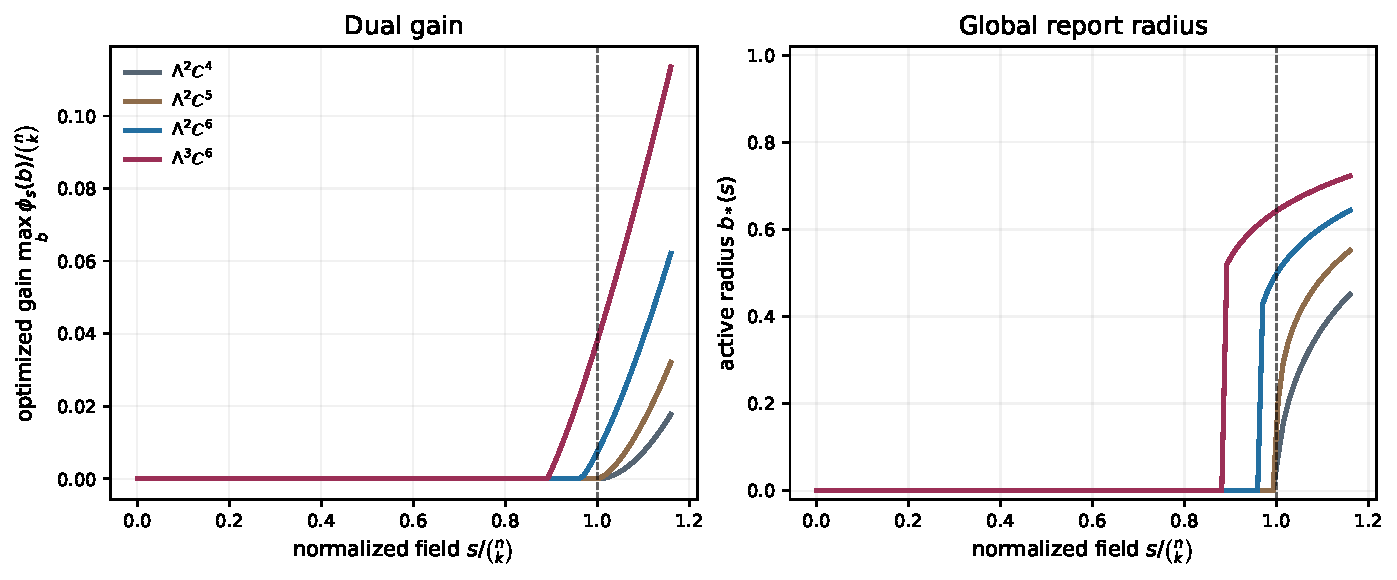
\includegraphics[width=.82\textwidth]{coherent_orbit_envelopes.pdf}
\caption{Scalar dual envelope for representative phased Slater families.
The plotted quantity is $\max_b\phi_s(b)$; dots mark the local stability
field $s_0=\binom nk$.  Interior families with $n\ge6$ already have a
positive-radius global phase at $s_0$, as proved by
\cref{thm:slaterphase}.  The plot is diagnostic and is not used in any
proof.}
\label{fig:envelopes}
\end{figure}

\section{The phase-invariant quotient}

Global phase is part of the source in \cref{thm:rdf}.  When only the
projective coherent state matters, use the intrinsic Pl\"ucker distortion
\[
 \delta([x],[y])=1-|\ip{x}{y}|^2.
 \tag{8.1}
\]
Here reproduction is restricted to the same projective homogeneous space;
there is no radial orbitope report.

\begin{corollary}[Projective coherent-orbit frontier]\label{cor:projective}
Let $[X]$ be Haar on the compact projective highest-weight orbit
$G/K_\lambda\simeq G_\C/P_\lambda$, and put
$N=\dim V_\lambda$.  With reproduction restricted to this same orbit,
under (8.1),
\[
 R_\lambda^{\rm proj}(D)
 =\sup_{s\ge0}\left\{-sD+s-\log H_\lambda(s)\right\},
 \qquad
 H_\lambda(s)=\sum_{m=0}^\infty\frac{s^m}{m!d_m}.
 \tag{8.2}
\]
for $0<D<1-1/N$.  Moreover
$R_\lambda^{\rm proj}(D)=0$ for $D\ge1-1/N$, and the value at $D=0$ is
the limiting value $+\infty$ for a positive-dimensional orbit.  For
$\Gr_\C(k,n)$, substitute (7.1).
\end{corollary}

\begin{proof}
For fixed $[y]$, invariance makes
\[
 \E e^{-s\delta([X],[y])}
 =e^{-s}\E e^{s|\ip{X}{y}|^2}
 =e^{-s}H_\lambda(s)
\]
independent of $[y]$.  The constant Shannon dual is therefore feasible,
and the covariant exponential reverse channel has the Haar source marginal
and saturates it.  Its distortion is
$D(s)=1-H_\lambda'(s)/H_\lambda(s)$; strict log-convexity makes $D(s)$
continuous and strictly decreasing from $1-1/N$ to zero, so every stated
interior distortion is covered.  This is the same invariant-partition
mechanism used for compact groups \cite{Harremoes2009}, applied here directly
to the transitive projective orbit; the explicit dimension sequence is the
representation-theoretic specialization.
\end{proof}

The quotient result answers an intrinsic subspace-compression question.  It
must not be conflated with \cref{thm:rdf}, whose decoder may report any point
of the orbitope and whose radial shrinkage causes coexistence.

\section{Reproducibility and claim boundaries}

The lightweight replay accompanying this paper checks:
\begin{itemize}
\item 728 exact rectangular-dimension and Hodge-complement identities;
\item the hook identity (7.4) and every quartic sign for $n\le12$;
\item the exceptional cumulants, including $-1/11200$ at $(5,2)$;
\item the $k=1$ ${}_0F_1$ reduction to relative error below
$2.1\times10^{-15}$;
\item representative high-field constants and scalar activation
diagnostics.
\end{itemize}
These checks replay algebra and numerics; they do not certify
\cref{lem:cartan,thm:rdf} or the uniform saddle proof.  Those arguments are
analytic and are stated in full above.

Several boundaries are essential.  First, the integer moment maximization
is due to Sugita; our new use is the all-field transform and exact classical
RDF.  Second, the phase-lifted source is a classical random amplitude vector.
It is not a quantum message, so no quantum coding rate is claimed.  Third,
the squared ambient distortion is not click-only Born calibration.  Fourth,
the discontinuity criterion proves a first coexistence event but not a
universal one-fold or no-reentrance theorem.  Finally, the intrinsic quotient
corollary restricts reproduction to the homogeneous space and is formally a
different operational problem.

\section{Conclusion}

The Cartan product turns a large family of apparently high-dimensional
compression problems into one scalar envelope.  The key geometric fact is
simultaneous: coherent rays maximize every integer overlap moment and hence
the complete Laplace transform at every field.  Conditional means and
Shannon duality then promote that rigidity to an exact unrestricted
rate--distortion theorem for every phase-lifted generalized coherent-state
orbit.

Representation theory remains visible in the operational answer.  The full
dimension sequence $\dim V_{m\lambda}$ is the scalar partition function;
$\dim V_{2\lambda}$ decides whether directional information turns on
discontinuously; positive roots determine the exact high-fidelity offset.
For fermionic Slater determinants these data become elementary rectangular
dimensions, a beta-product overlap, and a sharp all-$(n,k)$ transition
criterion.  This higher-exterior-degree family is qualitatively broader than
a single Grassmannian or low-rank spectral case while retaining a complete,
falsifiable formula.

The natural next problem is phase-diagram rigidity: identify highest weights
for which the scalar radial envelope has a unique positive branch and no
reentrance.  That question is not needed for the exact frontier proved here,
and it remains open outside special dimension sequences.

\section*{Data and code availability}

The source package contains the LaTeX manuscript, bibliography, the bounded
Python replay, its JSON output, and the figure-generation script.  No
external data set is used.  All floating-point output is diagnostic; the
theorems do not depend on numerical optimization.

\section*{Use of AI tools}

AI tools assisted with literature discovery, algebraic replay, drafting, and
adversarial checking.  The named author takes responsibility for the claims,
proofs, citations, and release artifacts.  No peer review or independent
experimental validation is claimed.

\printbibliography

\end{document}
